\documentclass[11pt,a4paper]{article}
        \usepackage[margin=2.2cm]{geometry}
        \usepackage{graphicx}
        \usepackage{float}
        \usepackage{parskip}
        \usepackage{amsmath}
        \title{Xarray for CHGCAR and DOSCAR in OnePiece}
        \author{Claude Coppex}
        \date{June 8, 2026}
        \begin{document}
        \maketitle
        This homework-style report explains how \texttt{xarray} is used inside OnePiece to analyze labeled three-dimensional charge-density fields and energy-resolved density-of-states data from VASP. The emphasis is on scientifically meaningful labeled reductions rather than on general plotting alone.
        \clearpage
        \section*{Why xarray is useful for CHGCAR}
The CHGCAR reader gives a three-dimensional scalar field. In OnePiece, xarray adds named axes, coordinate values at voxel centers, and metadata describing the simulation cell and atom positions. This makes later reductions and selections much easier to read and to validate.

\begin{figure}[h]
\centering
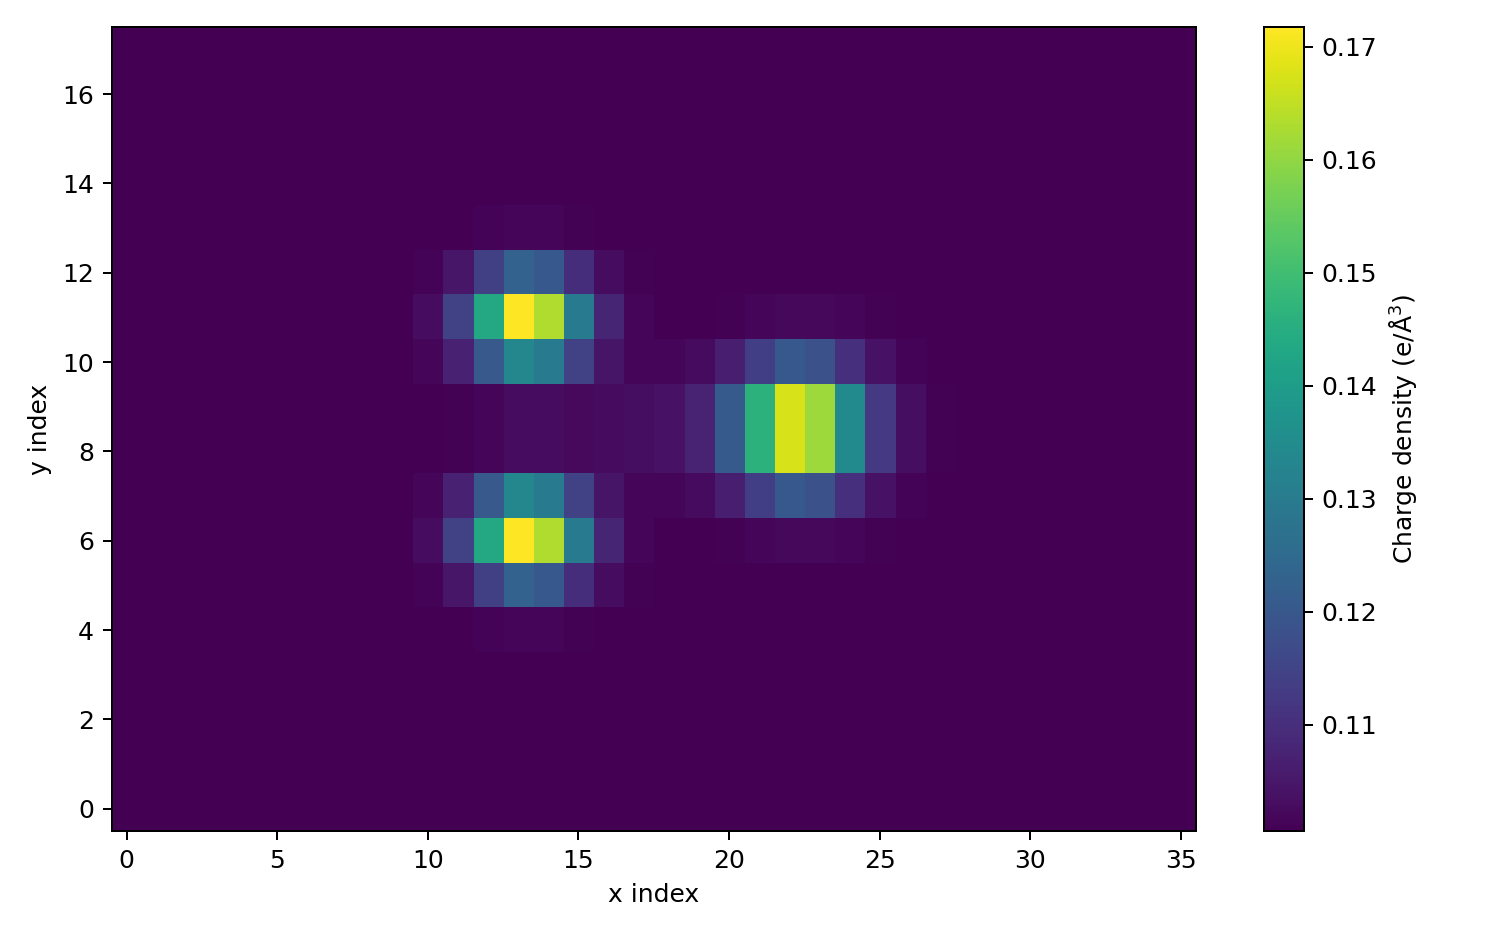
\includegraphics[width=0.92\textwidth]{assets/page_01_charge_density_slice.png}
\caption*{Charge density slice from CHGCAR as a labeled xarray field}
\end{figure}
\clearpage

\section*{Multiple variables in one dataset}
Charge density and spin density share the same grid. xarray keeps both variables in one dataset with the same coordinates, which is more natural than carrying several unrelated ndarrays.

\begin{figure}[h]
\centering
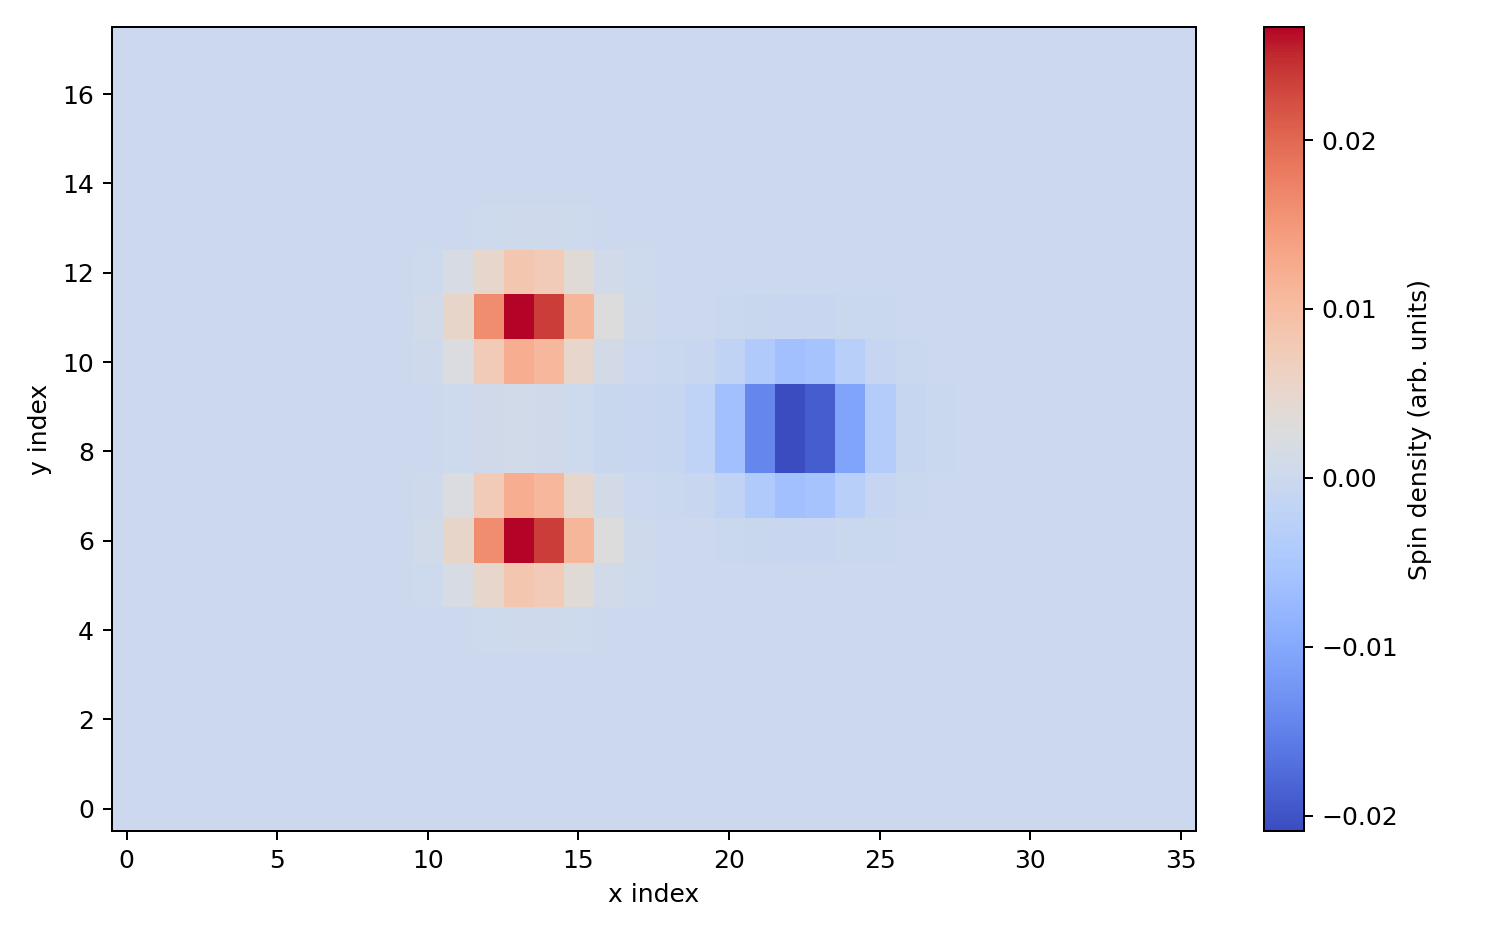
\includegraphics[width=0.92\textwidth]{assets/page_02_spin_density_slice.png}
\caption*{Spin-density slice from the same grid using an additional data variable}
\end{figure}
\clearpage

\section*{Planar averages}
A planar average is a named-dimension reduction over x and y. This is a common slab-analysis step because the remaining z coordinate follows the surface normal.

\begin{figure}[h]
\centering
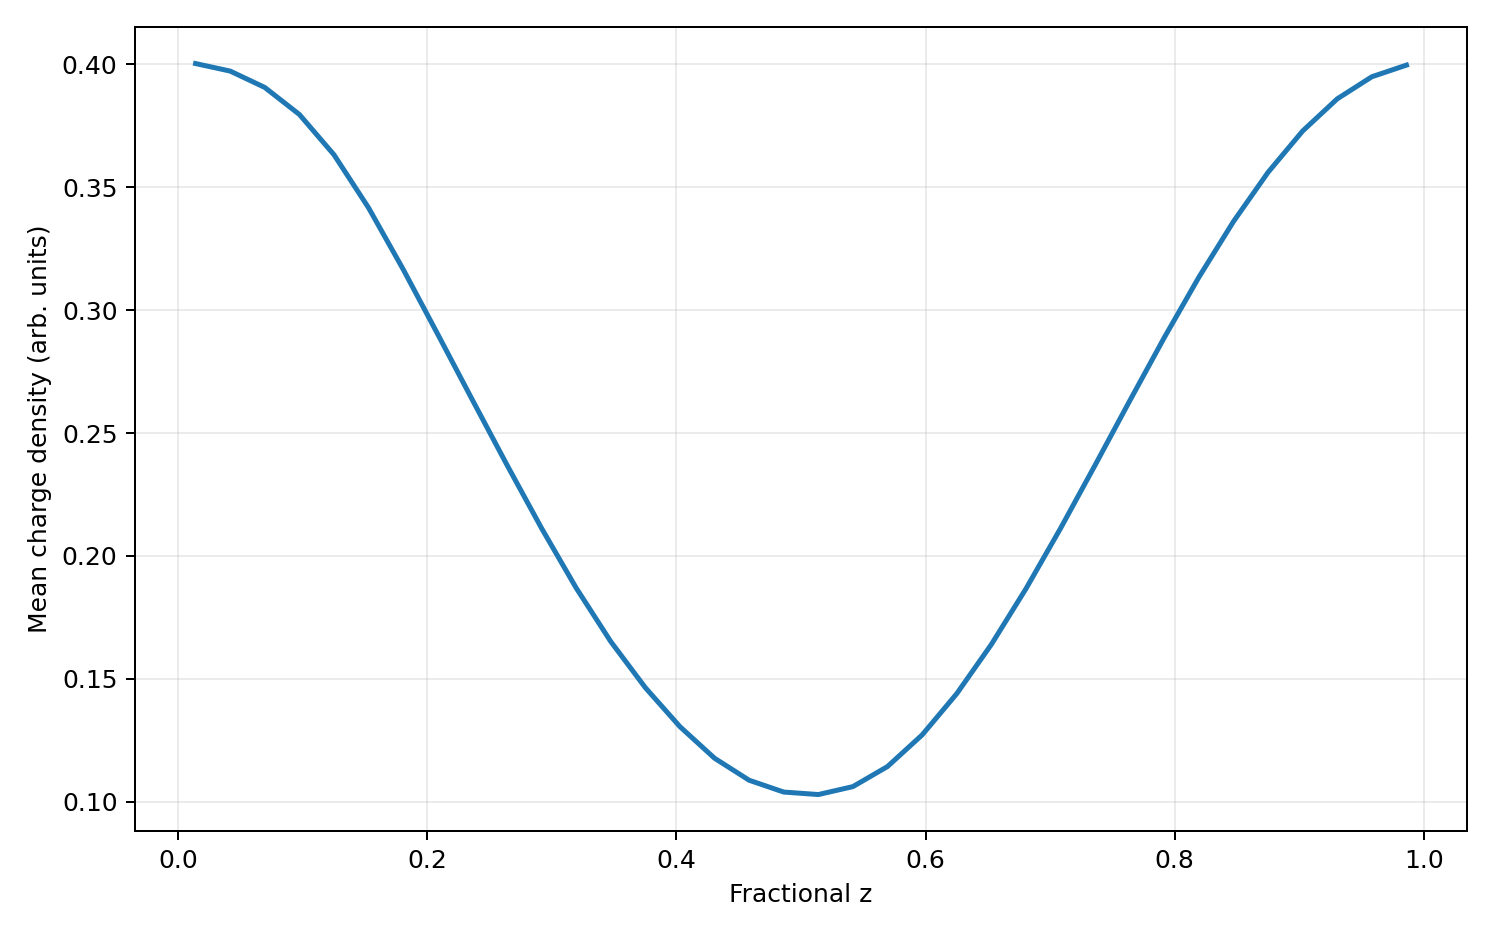
\includegraphics[width=0.92\textwidth]{assets/page_03_planar_average.png}
\caption*{Planar average along z computed by averaging over x and y}
\end{figure}
\clearpage

\section*{Charge per slice}
Summing density over a plane and multiplying by voxel volume yields electrons per slice. The xarray-based helper keeps the axis label and therefore remains self-explanatory in later code.

\begin{figure}[h]
\centering
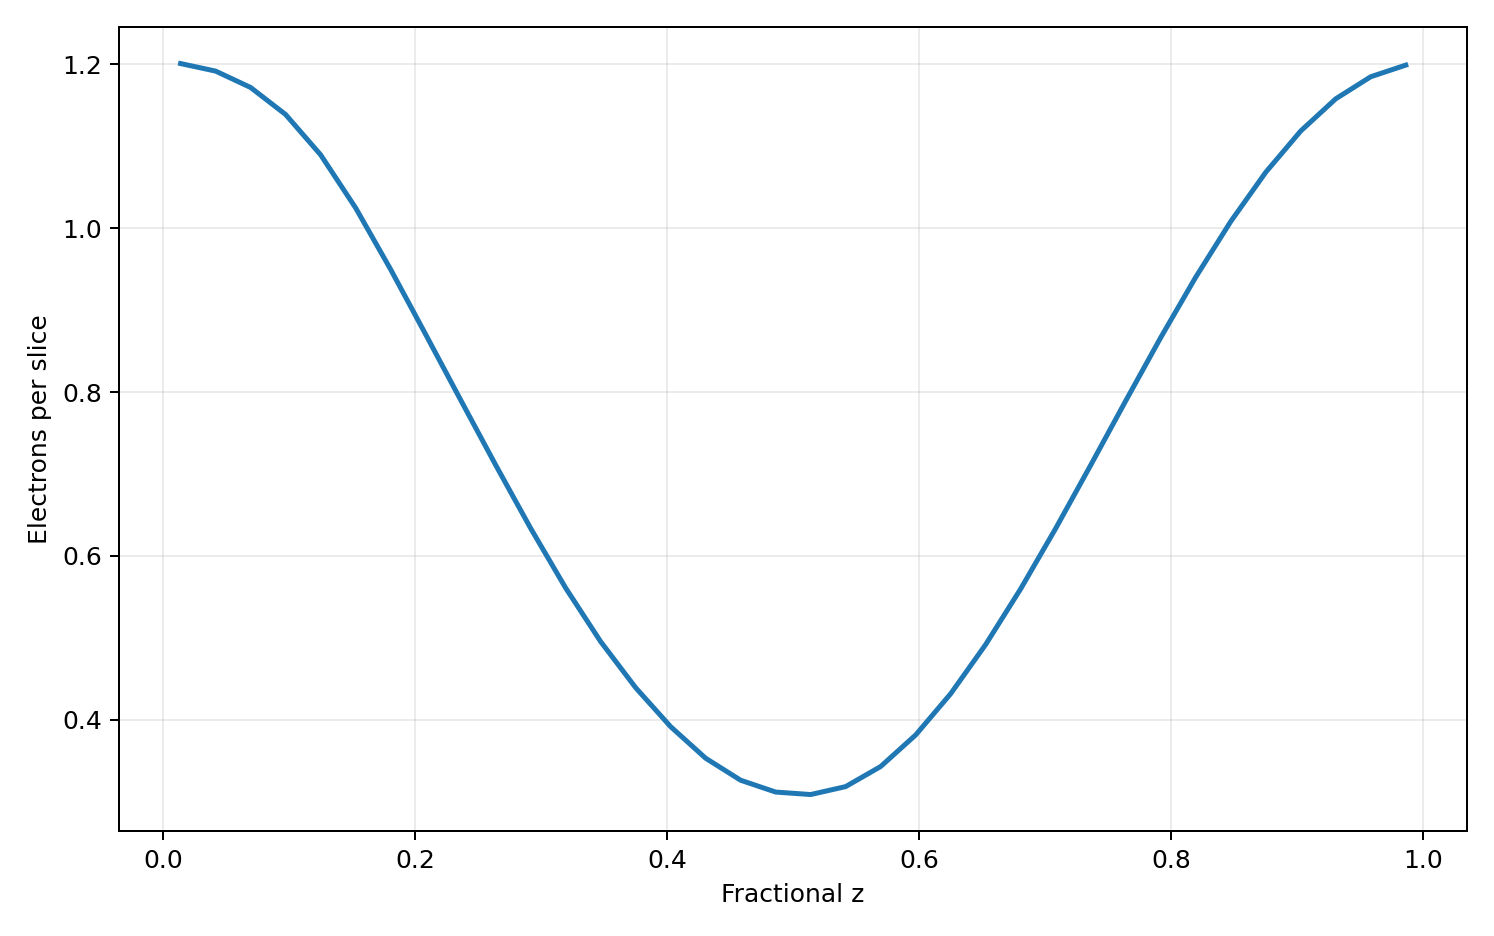
\includegraphics[width=0.92\textwidth]{assets/page_04_plane_electrons.png}
\caption*{Electrons per z-slice from density summation times voxel volume}
\end{figure}
\clearpage

\section*{Cumulative electron profile}
The cumulative profile integrates the slice electrons along z. It is useful for seeing how much electronic population lies below or above an interfacial region.

\begin{figure}[h]
\centering
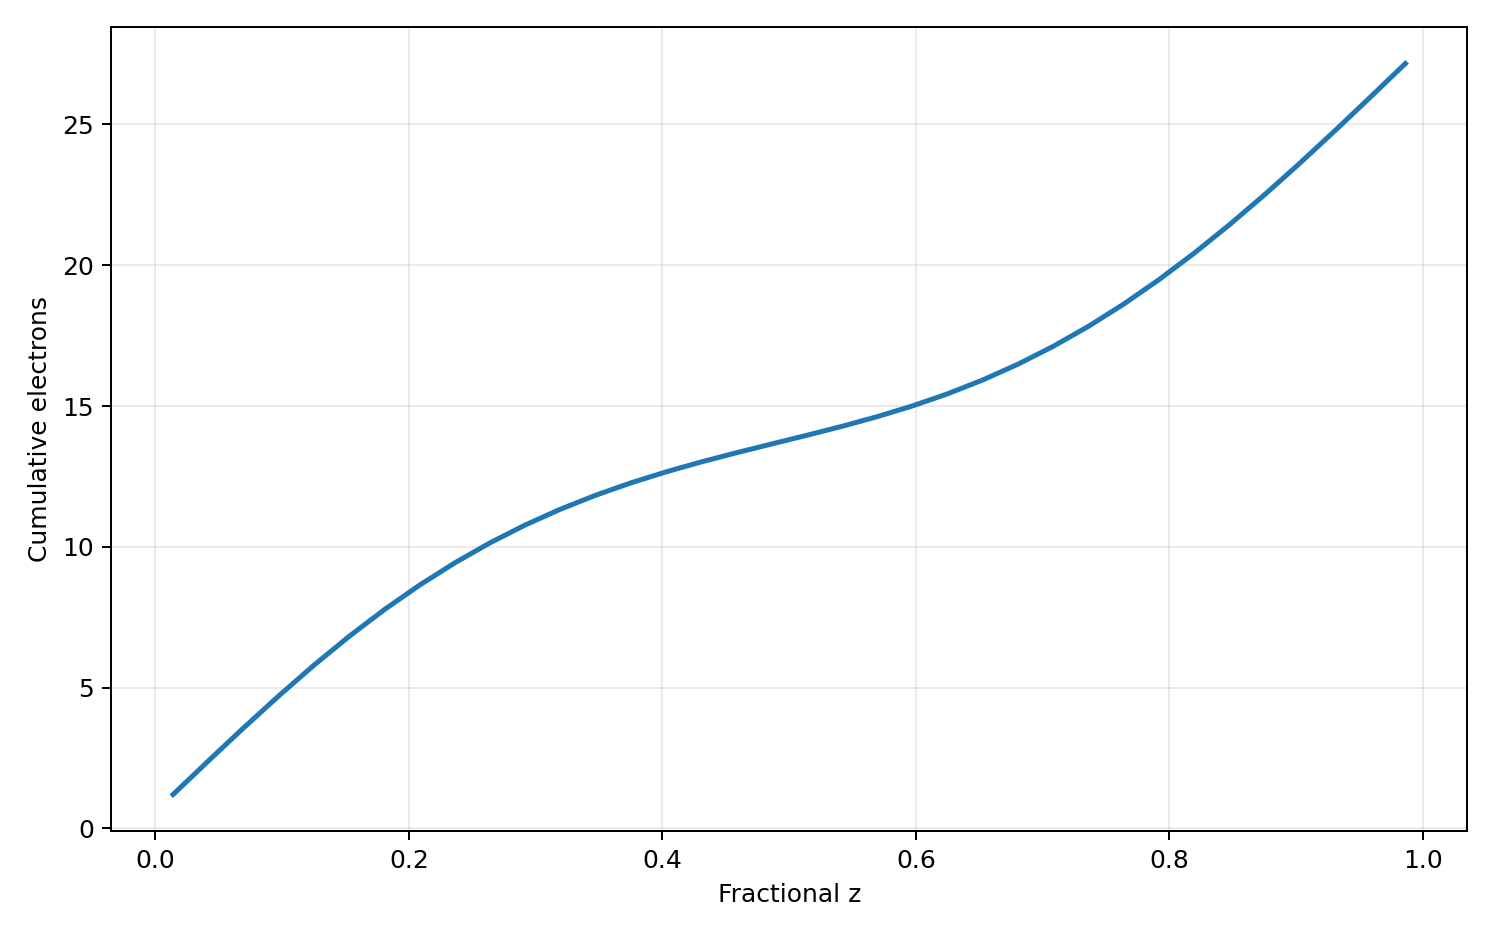
\includegraphics[width=0.92\textwidth]{assets/page_05_cumulative_profile.png}
\caption*{Cumulative electron profile that tracks where charge accumulates through the slab normal}
\end{figure}
\clearpage

\section*{Interpolated line profile}
A catalytic analysis often needs a profile along a bond axis or through an adsorption site. The line-profile helper samples the 3D field between two fractional points and returns both the sampled values and the traveled distance in angstrom.

\begin{figure}[h]
\centering
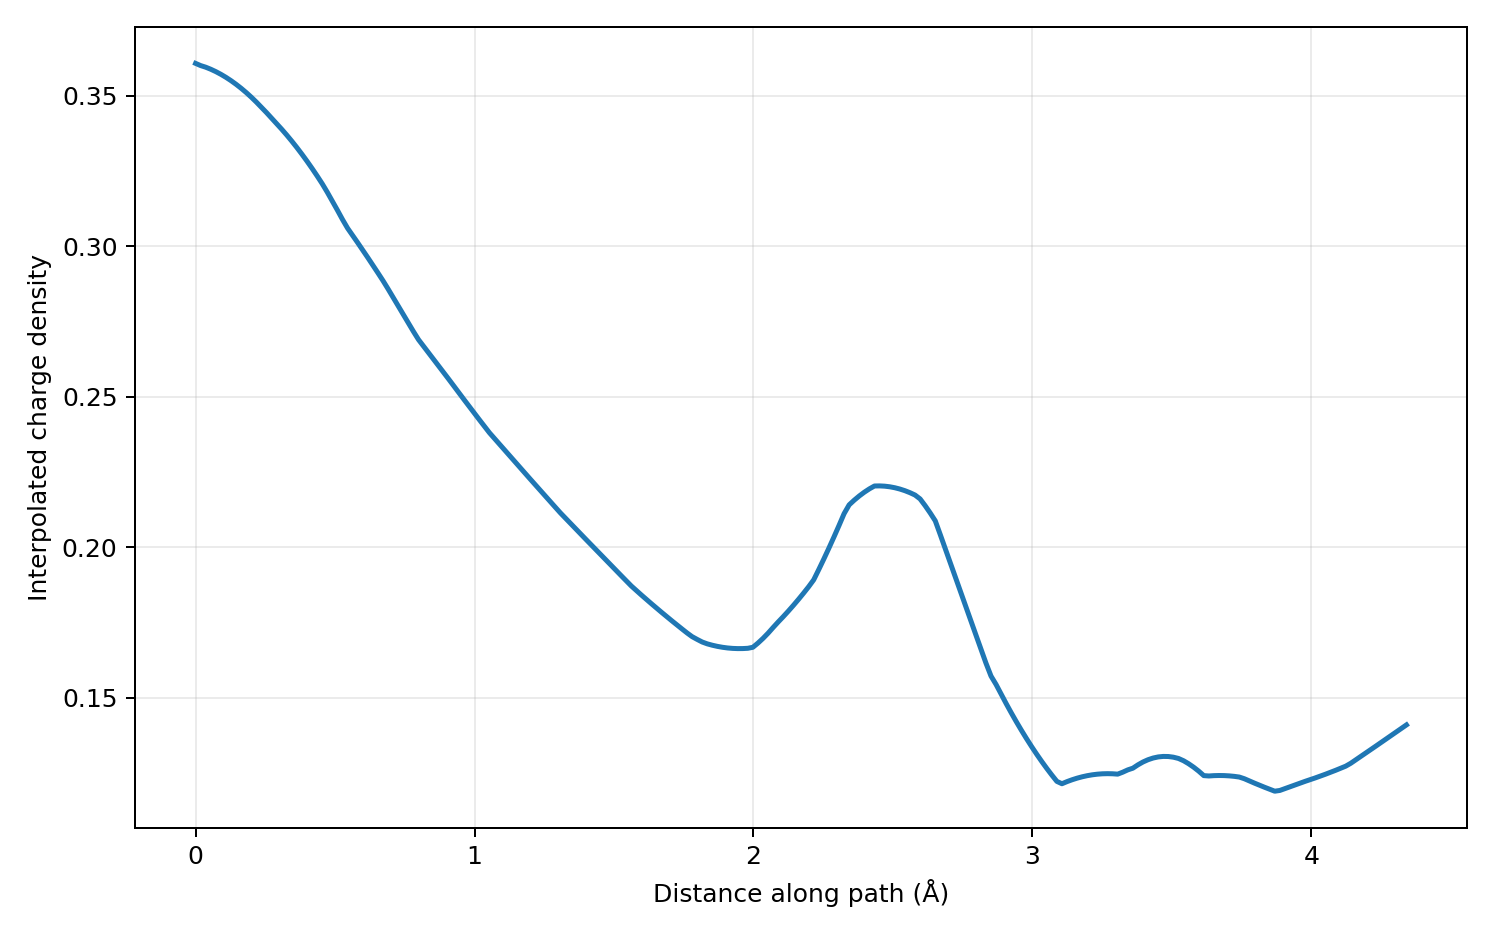
\includegraphics[width=0.92\textwidth]{assets/page_06_line_profile.png}
\caption*{Line interpolation through the 3D CHGCAR grid in fractional coordinates}
\end{figure}
\clearpage

\section*{DOSCAR as a labeled energy dataset}
For DOSCAR, xarray treats energy as the primary scientific coordinate. Total DOS and integrated DOS become energy-indexed observables instead of anonymous columns.

\begin{figure}[h]
\centering
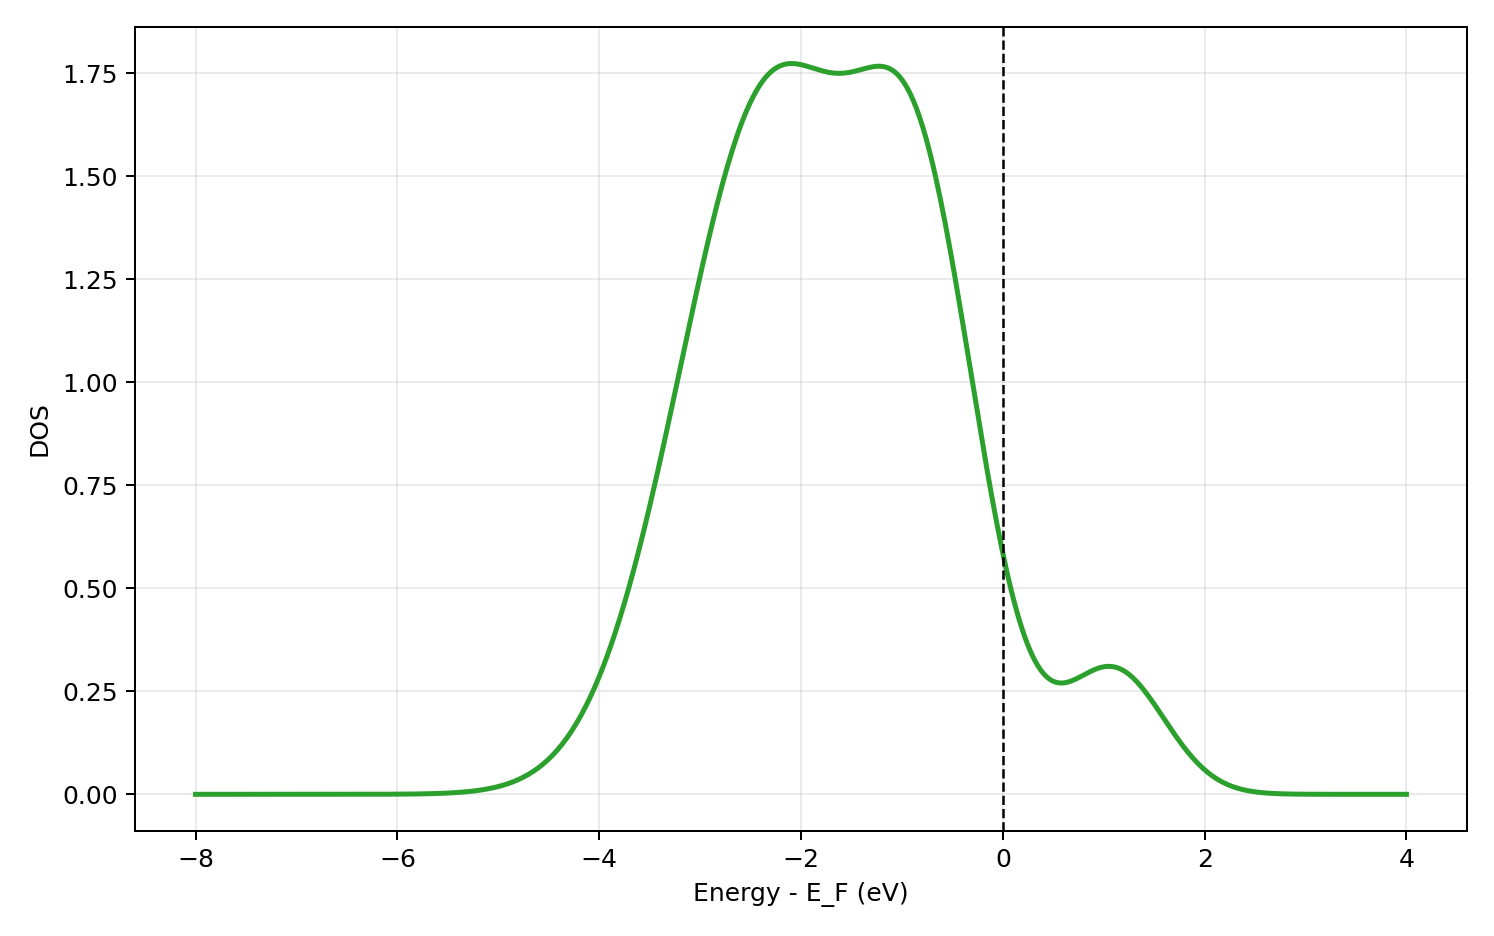
\includegraphics[width=0.92\textwidth]{assets/page_07_total_dos.png}
\caption*{Total DOS with an energy coordinate referenced to the Fermi level}
\end{figure}
\clearpage

\section*{Integrated DOS}
The integrated total DOS remains useful as a sanity check because it reflects the cumulative state count. The explicit energy coordinate also makes energy-window selection transparent.

\begin{figure}[h]
\centering
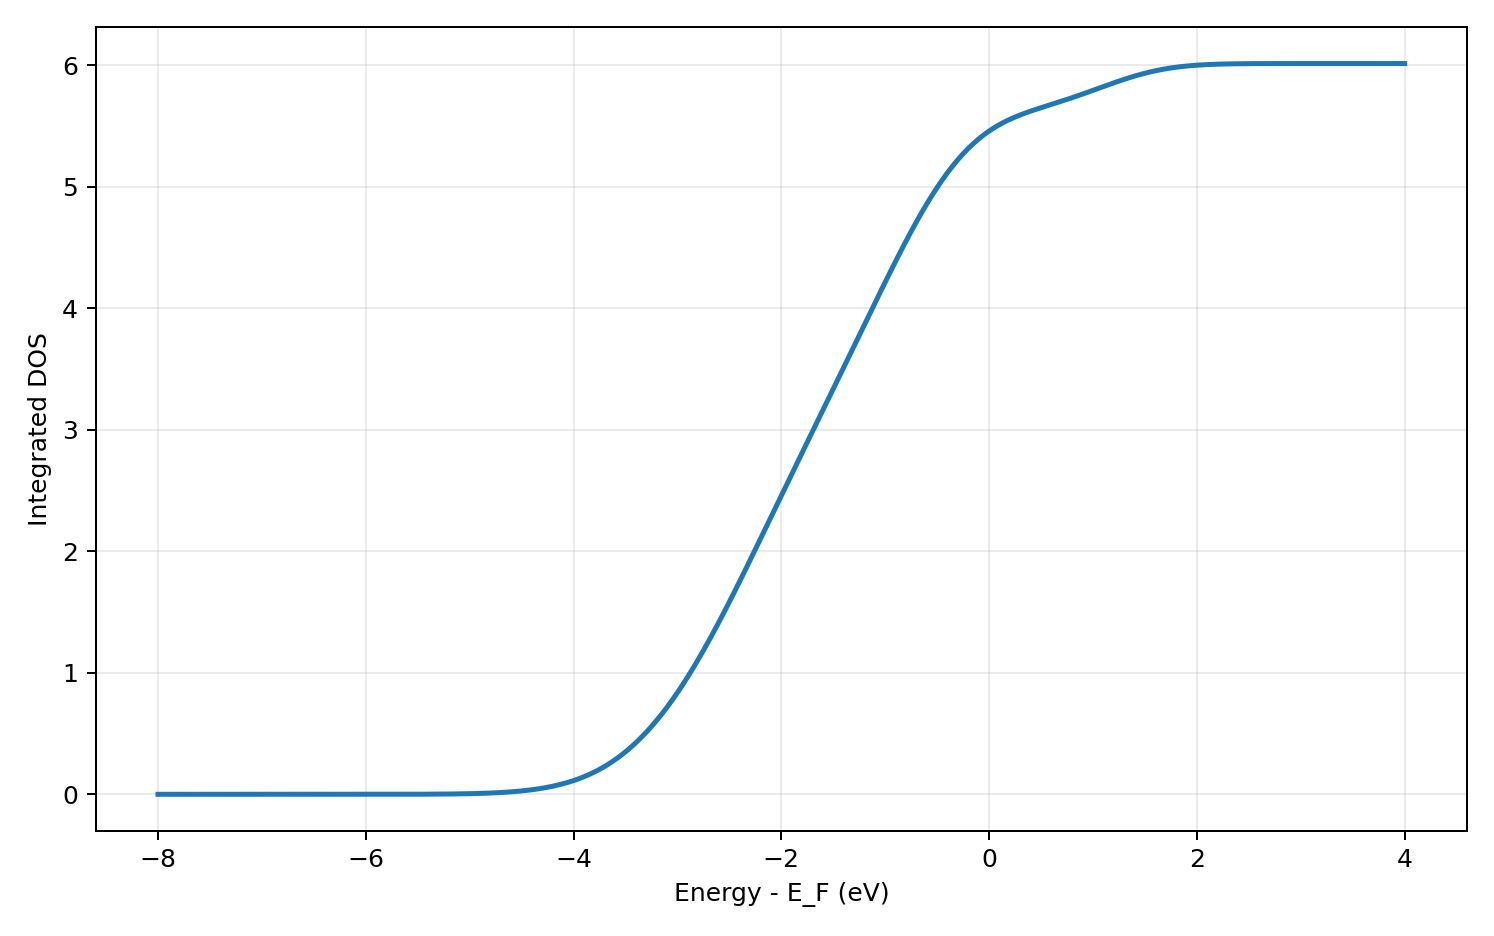
\includegraphics[width=0.92\textwidth]{assets/page_08_integrated_total_dos.png}
\caption*{Integrated total DOS as an energy-ordered cumulative observable}
\end{figure}
\clearpage

\section*{Atom- and orbital-resolved PDOS}
Projected DOS adds atom and orbital dimensions. This is where xarray is especially convincing because atom and orbital selections stay readable and composable.

\begin{figure}[h]
\centering
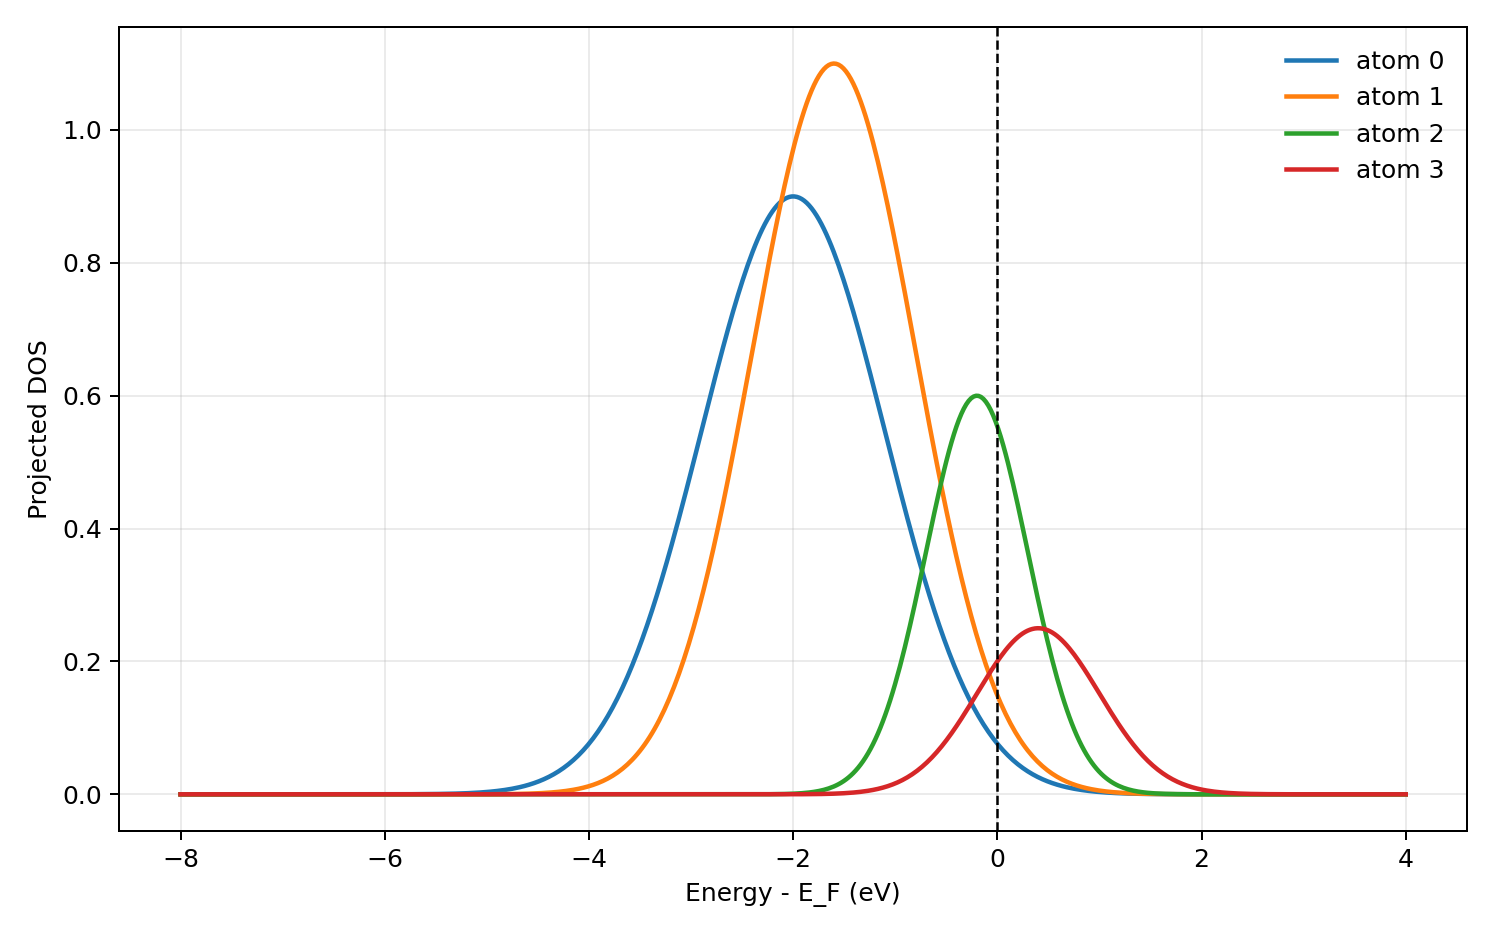
\includegraphics[width=0.92\textwidth]{assets/page_09_atom_resolved_d_pdos.png}
\caption*{Atom-resolved d-projected DOS extracted from the orbital dimension}
\end{figure}
\clearpage

\section*{d-band centers from selected subspaces}
A final practical descriptor is the d-band center. In OnePiece, it is derived from an xarray-selected PDOS subspace, which makes the calculation traceable: first choose atom and orbital labels, then integrate over the chosen energy range.

\begin{figure}[h]
\centering
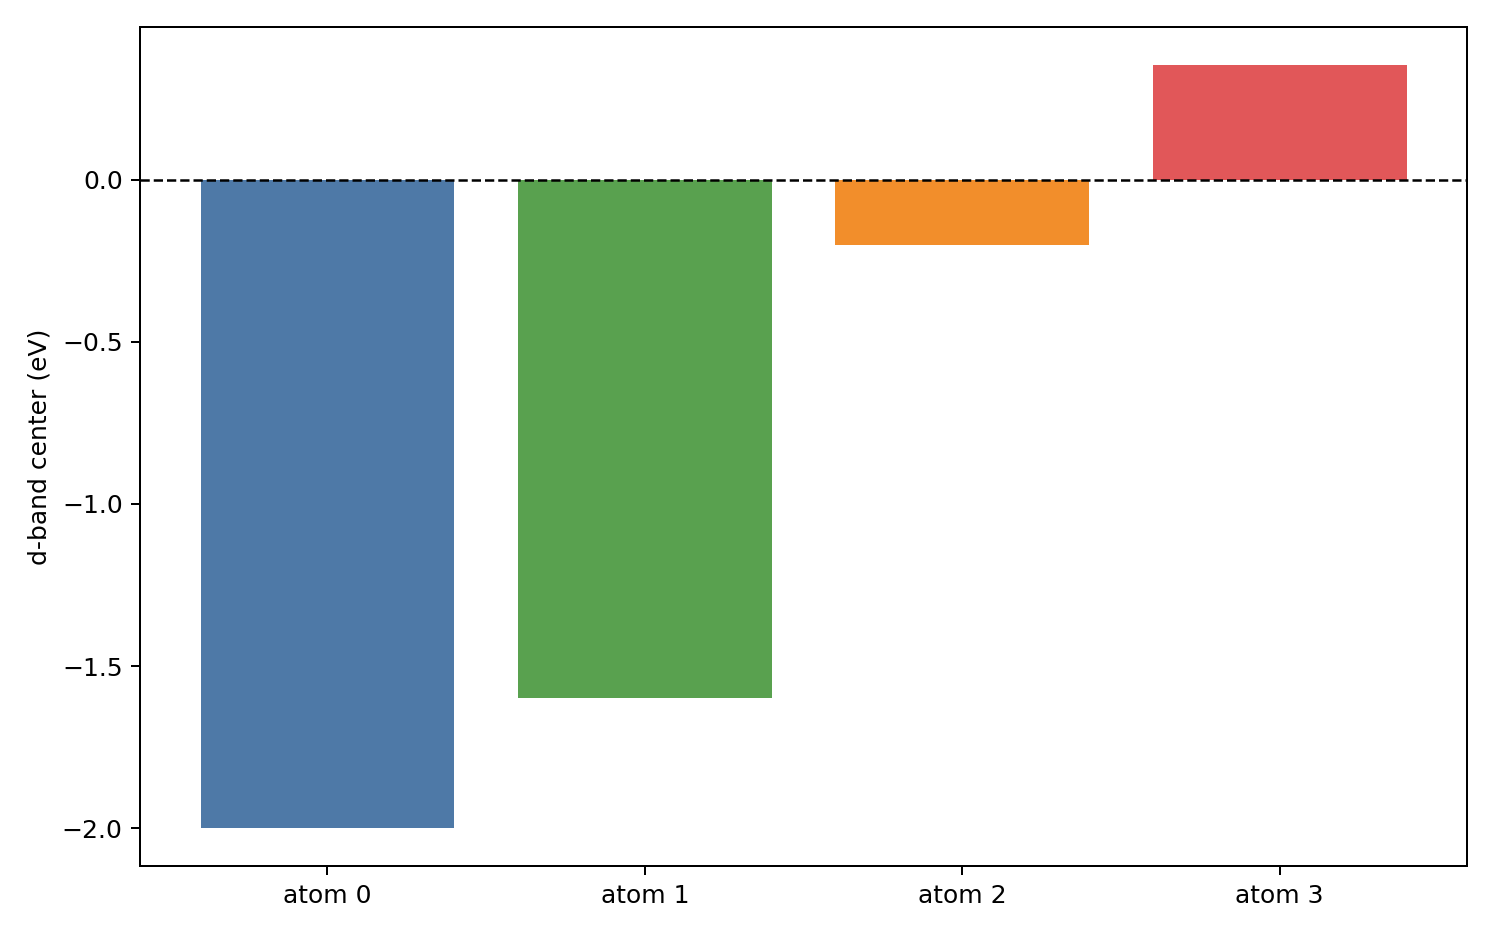
\includegraphics[width=0.92\textwidth]{assets/page_10_band_centers.png}
\caption*{d-band centers from xarray-selected atom and orbital subspaces}
\end{figure}
\clearpage
        \end{document}
